\chapter{Hajautettu järjestelmä}
\label{ch:distributed-systems}


\section{Mikä on hajautettu järjestelmä?}
\emph{Hajautettu järjestelmä} (engl. \emph{distributed system}) on verkko toisiinsa kytkettyjä fyysisiä- tai ohjelmistopohjaisia komponentteja, jotka kommunikoivat toistensa kanssa viestien välityksellä. Hajautetussa järjestelmässä osapuolten etäisyydellä ei ole merkitystä. Niiden välimatka voi olla eri maa tai sama rakennus. Hajautetut järjestelmät ovat oma tieteenala joka lähti liikkeelle käyttöjärjestelmien arkkitehtuurien tutkimuksista 1960-luvulla \cite[s.~384]{andrews2000foundations}. Ensimmäinen laajalle levinnyt hajautettu järjestelmä oli lähiverkot (engl. Local Area Network tai LAN), joka keksittiin 1970-luvulla \cite[s.~32]{andrews2000foundations}. Hajautetun järjestelmän määrityksistä ja toteuttamisesta on nykypäivänä olemassa hyvin kirjallisuutta ja tietoa, esimerkiksi \cite{distributed-systems-concepts-and-design, distributed-event-based-systems, mullender1993distributed, baldoni2005distributed}.

Järjestelmän hajautuksessa ja sen käytössä on pääasiassa kyse resurssien jakamisesta osapuolien kesken. Resurssi on abstrakti käsite ja voi tarkoittaa tekniikasta tai toteutuksesta riippuen montaa eri asiaa. Resurssilla voidaan esimerkiksi kuvata jaettua fyysistä laitetta kyten levyä tai tulostinta, ohjelmiston tapauksessa oliota tai tietokantaa \cite[s.~2--3]{distributed-systems-concepts-and-design}. Nykyinen internet mahdollistaa monien eri laitteiden kytkemisen verkkoon ja niiden kommunikoinnin keskenään, ja on nykypäivänä hyvä esimerkki todella laajasta hajautetusta järjestelmästä.

Hajautetussa järjestelmässä voidaan puhua osapuolten \emph{heterogeenisyydestä} (engl. \emph{heterogeneity}), eli osapuolet voivat kommunikoida toistensa kanssa tekniikasta tai toteutuksesta riippumatta. Tämä voidaan kuvata kerrosarkkitehruurin avulla. Korkean ja matalan tason ohjelmistojen välissä on ns. \emph{väliohjelmistokerros} (engl. \emph{middleware}). Tämän kerroksen tehtävä on abstrahoida matalan tason ohjelmisto tai alusta ja tehdä siitä heterogeeninen ylemmän tason ohjelmistoille ja palveluille. Kuvassa \ref{fig:middleware-architecture} on esitetty edelle mainittu kerrosarkkitehtuuri. \mbox{\cite[s. ~16--17]{distributed-systems-concepts-and-design}} \mbox{\cite[s.~2--3]{distributed-event-based-systems}}

\begin{figure}[ht!]
	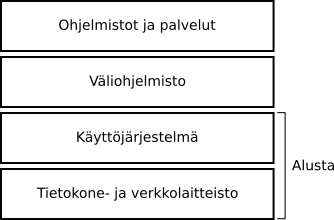
\includegraphics[width=0.5\textwidth]{pictures/middleware-architecture.png}
	\caption{Väliohjelmistokerros abstrahoimaan alusta heterogeeniseksi ylemmän tason ohjelmistolle (pohjautuu kuvaan \mbox{\cite[s.~52]{distributed-systems-concepts-and-design}}).}
	\label{fig:middleware-architecture}
\end{figure}


\subsection{Kuinka osapuolet kommunikoivat?}
Hajautetussa järjestelmässä osapuolet kommunikoivat keskenään viestien välityksellä. Jotta viestit voitaisiin vaihtaa tekniikasta riippumattomasti osapuolten välillä, täytyy tieto esittää alustariippumattomassa muodossa. Kommunikoivien osapuolten täytyy sopia yhteisestä viestin formaatista. Ohjelmat yleensä käsittelevät tietoa ohjelmistokielen tarjoamilla tietorakenteilla kuten esimerkiksi listoilla, puurakenteilla ja luokilla. Jotta tieto saadaan lähetettyä viestinä, täytyy se ensin muuntaa lähetykseen sopivaan muotoon. Tämä prosessi tunnetaan englannin kielellä nimellä \emph{marshalling}. Jotta vastaanotettua tietoa voidaa käyttää, täytyy viesti purkaa takaisin ohjelmistokielen rakenteiksi. Tämä prosessi englannin kielessä tunnetaan nimellä \emph{unmarshalling}. \mbox{\cite[s.~158]{distributed-systems-concepts-and-design}}

Kommunikointiin voidaan osapuolten välillä sopia erilaisista takuita lähetyksistä ja tiedon oikeudesta. Lähettäjä voi esimerkiksi vaatia vastaanottajaa kuittaamaan viestin vastaanottamisen. Jos kuittausta ei tule tietyn ajan sisällä, lähettäjä uudelleenlähettää viestin vastaanottajalle. Esimerkki tästä on TCP-protokollan (engl. Transmission Control Protocol) paketit, jossa lähettäjä odottaa vastaanottajan kuittausta paketista \cite[s.~9--10]{tcp-standard}. On myös tilanteita jossa lähettäjä ei välitä saako vastaanottaja viestin. Tässä tapauksessa osapuoli lähettää viestejä ilman tietoa siitä ottaako niitä kukaan vastaan. Esimerkki tästä on UDP-prokollan (User Datagram Protocol) paketit jossa lähettäjä ei odota kuittausta paketteihin \cite{udp-standard}. Uuden onnistuneesti lähetetyn paketin odotetaan korvaavan entisen tieto. Minkälainen takuu viestien lähetykseen valitaan riippu ohjelmiston vaatimuksista.


\subsection{Kommunikoinnin luokittelu}
\label{ch:liitokset}
Hajautetuissa järjestelmissä osapuolten kommunikoinnin välillä voi olla \emph{suora-} tai \emph{epäsuora liitos}. Suora liitos tarkoittaa tilannetta, jossa osapuolet tietävät toistensa identiteetin. Esimerkiksi lähettäjä lähettää viestiin suoraan vastaanottajalle. Epäsuora liitos tilannetta jossa osapuolet eivät tiedä toistensa identiteettiä. Epäsuorassa liitoksessa osapuolet yleensä kommunikoivat välittäjän kautta, joka hoitaa viestien lähettämisen toiselle osapuolelle. Suorassa liitoksessa toisen osapuolen vaihtaminen on vaikeampaa kuin epäsuorassa liitoksessa. Esimerkkinä tästä on yksinkertainen asiakas-palvelin-malli. Suoran liitoksen takia palvelin on vaikeampi vaihtaa toiseen samanlaiseen (palvelin tulkkaa HTML-sivuja asiakkalle). Epäsuorassa liitoksessa palvelimen vaihto samanlaiseen on helpompaa jos niiden välissä on tarpeeksi epäsuoruutta (geneerinen rajapinta tai välittäjä). \cite[s.~230]{distributed-systems-concepts-and-design}

Hajautetuissa järjestelmissä voidaan puhua erilaisista heikkojen liitoksien luokittelumalleista. Kirjallisuudessa näitä kutsutaan
\begin{itemize}
	\item \emph{heikko tilaliitos} (engl. \emph{space uncoupling}), tarkoittaa liitosta jossa osapuolet eivät tiedä toistensa identiteettiä, ja
	\item \emph{heikko aikaliitos} (engl. \emph{time uncoupling}), tarkoittaa liitosta jossa osapuolien ei tarvitse olla olemassa samaan aikaan.
\end{itemize}
Näiden mukaan voidaan esittää malli, jolla luokitellaan osapuolten välistä liitosta. Tämä malli on esitetty taulukossa \ref{tab:communication-models}. \cite[s.~230]{distributed-systems-concepts-and-design} \cite[s.~116]{eugster2003many}

\begin{table}[ht!]
	\caption{Hajautetussa järjestelmässä osapuolten kommunikoinnin luokittelun malli (pohjautuu taulukoihin \mbox{\cite[s.~231]{distributed-systems-concepts-and-design}} \mbox{\cite[s.~84]{cabri2000mobile}}).}
	\label{tab:communication-models}
	\begin{tabular}{p{0.1\linewidth} | p{0.37\linewidth} | p{0.37\linewidth}}
		\hline
		& \textbf{Vahva aikaliitos} & \textbf{Heikko aikaliitos} \\
		\hline
		\textbf{Vahva tilaliitos} & Kommunikointi tarkoitettu suoraan toiselle osapuolelle. Osapuolten täytyy olla olemassa samaan aikaan, esimerkiksi suora viestintä tai etäfunktiokutsu. & Kommunikointi tarkoitettu suoraan toiselle osapuolelle. Osapuolet voivat olla olemassa eri aikaan.\\
		\hline
		\textbf{Heikko tilaliitos} & Osapuolten ei tarvitse tietää toistensa identiteettiä. Osapuolten täytyy olla olemassa samaan aikaan, esimerkiksi IP-ryhmälähetys. & Osapuolten ei tarvitse tietää toistensa identiteettiä. Osapuolet voivat olla olemassa eri aikaan, esimerkiksi julkaisija-tilaaja ja viestijono \\
		\hline
	\end{tabular}
\end{table}

Taulukossa \ref{tab:communication-models} vasemmassa yläkulman luokittelu tarkoittaa kommunikointia, missä osapuolet tietävät toistensa identiteetin ja niiden täytyy olla olemassa samaan aikaan. Tämä on siis kaikista vahvin liitos mitä osapuolten välillä voi olla ja jossa on vähiten epäsuoruutta. Esimerkkinä tästä kommunikoinnista on etäfunktiokutsu tai suora viestintä prosesseiden välillä. Oikeassa yläkulmassa on tilanne, jossa osapuolet edelleen tietävät toistensa identiteetin, mutta niiden ei tarvitse olla olemassa samaan aikaan. Esimerkkinä osapuoli lähettää viestin tietylle identiteetille, mutta vastaanottaja ottaa viestin vastaan vasta myöhemmin. Teknistä esimerkkiä tähän tilanteeseen on hankalampi esittää kuin taulukon muihin kohtiin. Taulukon vasemmassa alakulmassa on tilanne jossa osapuolet eivät teidä toistensa identiteettiä, mutta niiden täytyy olla olemasa samaan aikaan. Esimerkkinä tästä on IP-ryhmälähetys, jossa viesti lähetetään kaikille verkon osapuolille ilman tietoa niiden identiteetistä. Vastaanottaja on olemassa samaan aikaan ja vastaa lähettäjälle ilman identiteettiä. Taulukon oikeassa alakulmassa on tilanne missä osapuolten välillä on kaikista eniten epäsuoruutta muista luokitteluista. Osapuolet eivät tiedä toistensa identiteettiä ja niiden ei tarvitse olla olemassa samaan aikaan. Esimerkkinä julkaisija-tilaaja- ja viestijono-paradigmat. \mbox{\cite[s.~230--232]{distributed-systems-concepts-and-design}} \mbox{\cite{cabri2000mobile}}

Epäsuoruus ohjelmoinnissa tuo hyötyjä ja joustavuutta ohjelmaan ja sen toimintaa kuten aikaisemmin tuotiin esille. Epäsuoruuden mukana tulee myös haittoja, kuten kommunikointi voi olla vaikeampaa osapuolten välillä ja epäsuoruus yleensä heikentää ohjelman suorituskykyä. Suorituskyky ja kommunikoinnin vaikeidet vaihtelevat tekniikasta ja toteutuksesta riippuen.

\section{Hajautuksen paradigmoja}
\begin{it}
	Lisätä tähän ongelmakohtaiset ja systeemikohtaiset osapuolet? Nyt on vain Ongelmakohtaiset osapuolet.
\end{it}
Hajautetussa järjestelmässä kommunikointi ja sen toteuttamisen mahdollisuudet ovat laajat ja vaihtoehtoja on paljon. Siksipä on tärkeää ymmärtää mitä ovat järjestelmän kommunikoivat osapuolet ja miten ne kommunikoivat. Näiden ymmärtäminen auttaa kehittäjää paremmin hahmottamaan vaihtoehtoja ja kokonaisuuden toimintaa.

Hajautetuissa järjestelmissä kommunikoivien osapuolien voidaan ajatella olevan \emph{olioita}, \emph{komponentteja} tai \emph{web-palveluita} (engl. \emph{World Wide Web}). Oliot tulevat suoraan olio-ohjelmoinnista ja on tarkoitettu jäsentämään asiaa tai toiminnallisuutta pienempiin omiin kokonaisuuksiinsa, joilla on oma sovittu rajapinta. Rajapinnan tarkoituksena on kapsuloida toiminnallisuutta helpokäyttöiseksi rajapinnaksi sen käyttäjälle. Komponenti on kokoelma olioita jotka muodostavat loogisen käytettävän kokonaisuuden. Komponenttit myös kommunikoivat rajapinnan läpi kuin oliot. Ero näiden välillä on, että komponentti oman rajapintansa lisäksi olettaa tiettyjä rajapintamäärityksiä muilta komponenteilta. Komponentti käyttää muiden komponenttien rajapintoja toteuttaaksen sille määritettyä toiminnallisuutta. Web-palvelut noudattavat samaa periaatetta rajapintojen kanssa kuin olio ja komponentti, mutta toimivat web-teknologioiden päällä. Olioita ja komponentteja käytetään toteuttamaan tiukemmin sidottuja ohjelmistoja. Web-palveluita käytetään toteuttamaan omia palvelukokonaisuuksia, joita voidaan liittää yhteen toteuttamaan kokonaisia applikaatioita. \mbox{\cite[s.~42--43]{distributed-systems-concepts-and-design}}

Hajautetussa järjestelmässä kommunikoinnin paradigmat voidaan jakaa kolmeen kategoriaan jotka on esitetty taulukossa \ref{tab:communication-paradigms}. Taulukossa tyyppien alla on esitetty sille tyypillisiä kommunikoinnin paradigmoja. Näitä paradigmoja käsitellään tarkemmin kappaleissa \ref{ch:interprocess-communication}, \ref{ch:remote-invocation} ja \ref{ch:indirect-communication}.

\begin{table}[ht!]
	\caption{Hajautetun järjestelmän kommunikointiparadigmat kolmella päätasolla (pohjautuu tauluun \mbox{\cite[s.~46]{distributed-systems-concepts-and-design}}).}
	\label{tab:communication-paradigms}
	\begin{tabular}{p{0.3\linewidth} | p{0.3\linewidth} | p{0.3\linewidth}}
		\hline
		\textbf{Prosessien välinen kommunikaatio} & \textbf{Etäkutsu} & \textbf{Epäsuora kommunikaatio} \\
		\hline \hline
		Viestien välitys (message passing) & Pyyntö-vastaus (request-reply) & Joukkokommunikointi (group communication) \\
		\hline
		Soketti (socket) & Etäproseduurikutsu (RPC) & Julkaisija-tilaaja (publish-subscribe) \\
		\hline
		Ryhmäkutsu (multicast) & Etämetodikutsu (RMI) & Viestijono (message queue) \\
		\hline
		& & Jonotaulu (tuple space) \\
		\hline
		& & Hajautetusti jaettu muisti (DSM) \\
		\hline
	\end{tabular}
\end{table}

\emph{Prosessien välinen kommunikointi} (engl. \emph{interprocess communication}) on matalan tason kommunikointia osapuolten välillä yleensä suoralla yhteydellä ohjelmointirajapintaan. \emph{Etäkutsut} (engl. \emph{remote invocation}) tarkoittavat toisen osapuolen kutsumista, joka suorittaa pyynnön ja palauttaa siihen vastauksen. Tyypillinen esimerkki tästä on asiakkaan pyyntö palvelimelle, johon palvelin lähettää takaisin vastauksen. Kahdessa aikaisemmin mainitussa kommunikoinnissa yhteistä on, että osapuolet tietävät eksplisiittisesti toistensa identiteetin ja niiden välillä on yleensä vahva aikaliitos. \emph{Epäsuora kommunikaatio} (engl. \emph{indirect communication}) tapahtuu kolmasta osapuolta käyttäen viestien välitykseen. Tämä mahdollistaa heikon liitoksen osapuolten välillä sekä ajallisesti että tilallisesti. Lähettäjä ei tiedä vastaanottajan identiteettiä ja toisin päin. Kolmas osapuoli vastaa viestin ohjaamisesta vastaanottajalle. \mbox{\cite[s.~43--45]{distributed-systems-concepts-and-design}}


\subsection{Prosessien välinen kommunikaatio}
\label{ch:interprocess-communication}
Prosessien välinen kommunikointi on matalan tason kommunikointia suoralla rajapinnan käytöllä. Esimerkkinä matalan tason kommunikoinnista on internet-protokollien käyttö, esimerkiksi UDP ja TCP. Käyttöjärjestelmät tarjoavat matalan tason rajapinnan kommunikointiin, esimerkiksi soketti-rajapinta. Soketti-rajapinnalla voidaan käyttää molempia UDP:tä ja TCP:tä \cite[s.~1152]{linux-programming-interface}. Tyypillistä tämän tason kommunikoinnille on että sen osapuolet tietävät toistensa identiteetin.

Käyttöjärjestelmän rajapintojen avulla prosessit voivat välittää viestejä suoraan toisilleen. Voidaan puhua, että prosessit lähettävät ja vastaanottavat toisilleen viestejä. Vastaanottaja toteuttaa yleensä jonon viestien vastaanottoon ennen käsittelyä. Jos kommunikointi on molemminsuuntaista, kummatkin osapuolet toteuttavat puskurin viestien vastaanottoon. Vastaanottaja voi kysellä tietoa jonosta toistuvasti saadakseen tiedon uudesta viestistä tai siitä voidaan keskeytyksellä. Viestien lähetys voi olla synkronista tai asynkronista. Synkronisessa viestien vaihdossa lähettäjä ja vastaanottaja sykronoidaan jokaisella viestillä. Eli viestin lähetys ja vastaanotto ovat pysäyttäviä (engl. blocking) operaatioita. Lähettäjän suoritus pysähtyy niin kauan kunnes vastaanottaja vastaa ja suoritus jatkuu. Asynkronisessa kommunikoinnissa operaatiot eivät ole pysäyttäviä (engl. non-blocking). Lähettäjä voi jatkaa muuta prosessointia heti kun viesti on kopioitu lähetyspuskuriin ja viestin lähetys jatkuu rinnakkain muun prosessoinnin kanssa. \mbox{\cite[s.~147--148]{distributed-systems-concepts-and-design}}

Hyviä puolia matalan tason kommunikoinnissa on, että sillä saadaan tehtyä saumaton kommunikointi prosessien välille ja sitä tukee moni nykyaikainen käyttöjärjestelmä. Matalan tason kommunikoinnin toteuttaminen vaatii paljon enemmän aikaa ja vaivaa ohjelmoijalta kuin korkeamman tason rajapinnan käyttö. Matalalla tasolla osapuolet ovat vahvasti liitoksissa ajallisesti ja tilallisesti. Osapuolet tietävät toistensa identiteetit ja niiden täytyy olla olemassa samaan aikaan. Vastaanottajan täytyy olla ottamassa vastaan viesti lähettäjältä samoihin aikoihin kun se lähetetään. Lisäksi matalantason ohjelma ei vältämättä ole modulaarinen ja on sidoksissa ympäristöönsä. Esimerkkinä Linux-käyt\-tö\-jär\-jes\-tel\-mäl\-le toteutettu ohjelma ei toimi Windows-käyttöjärjestelmällä. Tähän kuitenkin voidaan vaikuttaa ohjelman sisäisillä abstrahointitasoilla.


\subsection{Etäkutsu}
\label{ch:remote-invocation}
Etäkutsu paradigmoja ovat \emph{pyyntö-vastaus} (engl. \emph{request-reply}), \emph{etäproseduurikutsu} (engl. \emph{remote procedure call}, lyhennetään \emph{RPC}) ja \emph{etämetodikutsu} (engl. \emph{remote method invocation}, lyhennetään \emph{RMI}). Etäkutsuja voi suorittaa prosessit tai korkeamman tason objektit ja palvelut. Primitiivisin etäkutsu paradigmoista on pyyntö-vastaus, joka edustaa mallia aikaisemmin mainitun viestien välityksen päällä ja lisää siihen kaksisuuntaisen viestien vaihdon. Paradigmaa käytetään asiakas-palvelin kommunikoinnissa. \mbox{\cite[s.~185--186]{distributed-systems-concepts-and-design}}

Todella tärkeä määritys nykypäivän hajautettujen järjestelmien kannalta oli etäproseduurikutsut (RPC). Tämän määrittivät Birrell ja Nelson vuonna 1984 \cite{implemeting-remote-procedure-calls}. Se mahdollisti ohjelmoijan kutsua proseduuria toisella koneella etänä samoin kuin paikallista proseduuria. RPC-systeemi piilotti taustalle kaiken teknisen toteutuksen mitä kutsuun etänä tarvittiin, esimerkkinä tiedon siirron, pakkaamisen ja purkamisen \cite[s.~195--196]{distributed-systems-concepts-and-design}. Etämetodikutsu (RMI) toiminta on sama kuin RPC:n, mutta se on laajennettu toimivaksi olioilla. Olioiden metodeita voidaan kutsua niin kuin ne olisivat sen paikallisia metodeita \cite[s.~204]{distributed-systems-concepts-and-design}. Kummatkin RPC ja RMI tarjoavat saman tason abstraktion ohjelmoijalle ja piilottavat teknisen toteutuksen alleen.

Etäkutsuparadigmat ovat korkeamman tason paradigmoja kuin aikaisemmin mainittu prosessien välinen kommunikointi. Hyvänä puolena paradigmoissa on, että ohjelmoijan ei vältämättä tarvitse kirjoittaa matalan tason rajapinnan ohjelmaa. Rajapinta on abstrahoitu helppokäyttöisemmäksi ja sen toteutus ei vie niin paljon aikaa ja resursseja kuin matalan tason implementointi. Kuitenkin etäkutsut kärsivät samoista vahvoista liitoksista kuin prosessien väliset kutsut. Osapuolet ovat vahvasti liitoksissa ajallisesti sekä tilallisesti.


\subsection{Epäsuora kommunikaatio}
\label{ch:indirect-communication}
Epäsuora kommmunikaatio tarkoittaa osapuolten välistä kommunikaatiota välittäjän avulla. Osapuolet eivät vaihda tietoa suoraan keskenään ja eivät tiedä toisensa identiteettiä. Välittäjä huolehtii viestien reitittämisestä ja lähettämisestä vastaanottajalle. Välittäjän tarkempi toiminta ja tarkoitus vaihtelee toteutuksesta riippuen. Aikaisemmin mainittuissa kahdessa paradigmakategoriassa liitokset osapuolten välillä ovat pitkälti vahvoja ajallisesti sekä tilallisesti. Poikkeuksena tähän on esimerkiksi IP-ryhmälähetys, jossa osapuolilla on heikko tilaliitos, mutta vahva aikaliitos. Epäsuora kommunikointi osapuolten välillä vähentää liitoksien vahvuutta. Liitokset voivat olla heikkoja tilallisesti sekä ajallisesti ja niiden heikkous vaihtelee toteutuksesta riippuen. Epäsuora kommunikointi mahdollistaa toisen osapuolen helpomman vaihdon, siirron ja päivittämisen kuin suora kommunikointi. Useasti epäsuorassa kommunikoinnissa vastaanottajia voi olla monta yhden sijaan. Tällöin voidaan puhuta yksi-moneen-suhteesta (engl. one-to-many) osapuolten välillä. Epäsuoruus tuo hyötyjä, mutta se tuo myös väistämättöntä suorituskykykuormaa epäsuoruuden vaativan toiminnan takia. \mbox{\cite[s.~230--231]{distributed-systems-concepts-and-design}}

Epäsuoran kommunikoinnin paradigmoja ovat \emph{joukkokommunikointi} (engl. \emph{group communication}), \emph{julkaisija-tilaaja} (engl. \emph{publish-subscribe}), \emph{viestijono} (engl. \emph{message queue}), \emph{tuplesäilö} (engl. \emph{tuple space}) ja \emph{hajautetusti jaettu muisti} (engl. \emph{distributed shared memory}, lyhennetään \emph{DSM}). Nämä esitettiin aikaisemmin taulukossa \ref{tab:communication-paradigms}. Jokaista paradigmaa käsitellään erikseen tulevissa kappaleissa.

% TODO: Korjaa yllä oleva lause sitten kun on kirjoitettu loput kappaleet auki.


\subsection{Joukkokommunikointi}
Joukkokommunikointi on paradigma, jossa osapuoli lähettää viestin ryhmälle, jonka jälkeen viesti uudelleenlähetetään kaikille ryhmän osapuolille. Ryhmä vastaanottajia tunnistetaan yksilöivällä ryhmätunnisteella. Lähettäjä käyttää tunnistetta kohdentamaan viestin haluamalleen ryhmälle. Tässä tapauksessa lähettäjä ei ole tietoinen vastaanottajien identiteetistä \cite[s.~232--233]{distributed-systems-concepts-and-design}. Joukkokommunikointi tunnetaan myös \emph{joukkokommunikointisysteeminä} (engl. \emph{Group Communication System}, lyhennetään \emph{GCS}). Briman keksi ja kuvasi ensimmäinen tällainen systeemi 1986-luvulla \cite{isis-fault-tolerant-distributed-computing}. Joukkokommunikointi on tärkeä paradigma hajautettujen järjestelmien kannalta ja sillä on olemassa monta eri käyttökohdetta. Applikaatioina esimerkiksi voi olla kollaboraatio- ja monitorointi-ohjelmistot, jossa kaikkien osapuolien täytyy tietää uusimmasta muutoksesta.

Joukkokommunikoinnissa ryhmät voivat olla ns. avoimia tai suljettuja. Kuvassa \ref{fig:group-communication} on esitettu avoimen ja suljetun ryhmän toiminta. Avoin ryhmä mahdollistaa ulkopuolisen osapuolen lähettää viesti kaikille sen jäsenille. Suljettu ryhmä on tarkoitettu ainoastaan sen osapuolten väliseen kommunikointiin. Suljetussa ryhmässä yksi osapuoli voi ryhmälähettää viestin kaikille sen osapuolille ryhmän tunnisteella, samoin kuin ulkopuolinen avoimen ryhmän tapauksessa. Avoimen ja suljetun ryhmän lisäksi ryhmillä voi olla muitakin tärkeitä piirteitä. Ryhmät voivat olla päälekkäisiä tai ei päällekkäisiä. Päällekkäiset ryhmät mahdollistavat yhden osapuolen kuulua yhtä aikaa moneen ryhmään. Ei päälekkäisessä osapuoli voi kuulua enimmillään yhteen ryhmään. Joissakin tapauksissa ryhmän osapuolten voidaan sallia liittyä ja lähteä ryhmästä. Tällöin erillisen osapuolen täytyy pitää kirjaa ryhmän osapuolista ja tarjota toiminnallisuudet liittyä ja poistua ryhmästä. \mbox{\cite[s.~233--235]{distributed-systems-concepts-and-design}} \mbox{\cite[s.~48]{process-group-approach-briman}}

\begin{figure}[ht!]
	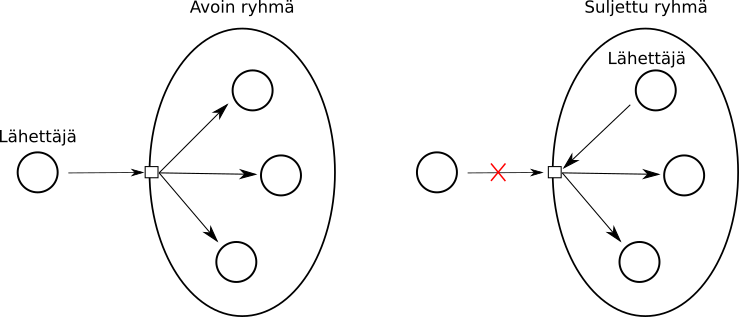
\includegraphics[width=1\textwidth]{pictures/group-communication.png}
	\caption{Osapuolten kommunikointi avoimessa ja suljetussa ryhmässä (pohjautuu kuvaan \mbox{\cite[s.~235]{distributed-systems-concepts-and-design}}).}
	\label{fig:group-communication}
\end{figure}

Ryhmät mahdollistavat yhden-moneen-suhteen kommunikoinnissa. Yksi viesti saadaan lähetettyä monelle osapuolelle yhdeltä kertaa. Tämä säästää kaistaa verrattuna tilanteeseen, jossa viesti lähetettäisiin jokaiselle osapuolelle erikseen. Joukkokommunikoinnissa osapuolten välillä on heikko tilaliitos, mutta vahha aikaliitos. Joukkokommunikointisysteemit ovat monimutkaisia ja niiden lähetystakuiden vaatimukset vaativat paljon vaivannäköä systeemiltä. Lähetystakuihin yleensä kuuluu että jokainen ryhmän jäsen saa sille lähetetyn viestin ainakin kerran jossakin vaiheessa. Dynaamisen ryhmän tapauksessa, jossa osapuolia voi tulle ja lähteä ryhmästä, lähetystakuiden kiinni pitäminen monimutkaistuu entisestään. \mbox{\cite{group-communication-specification}} \mbox{\cite[s.~236]{distributed-systems-concepts-and-design}}


\subsection{Julkaisija-tilaaja}
Julkaisija-tilaaja on kommunikointiparadigma, jossa \emph{julkaisijat} julkaisevat tapahtumia/viestejä ja \emph{tilaajat} tilaavat halumiaan tapahtumia/viestejä \emph{tilauksilla}. Osapuolten välissä on julkaisija-tilaaja-systeemi, joka vastaa viestien reitittämisestä tilaajille tehtyjen tilauksien perusteella. Järjestelmä mahdollistaa monen tilaajan tilata viestejä samalta julkaisijalta. Näin ollen kommunikointisuhde osapuolten välissä on yksi-moneen, kuten joukkokommunikoinnissa. Systeemiin tehdyllä tilauksella tilaaja voi tilata samalla kertaa monta eri julkaisijaa. Tehty tilaus on ns. \emph{suodatin/malli} (engl. \emph{pattern}), joka systeemin sääntöjen mukaan voi täsmätä enemmän kuin yhteen julkaistuun viestiin. Kirjallisuudessa paradigma tunnetaan nimellä \emph{julkaisija-tilaaja-systeemi} (engl. \emph{publish-subscribe system}) \cite{baldoni2005distributed}, sekä \emph{hajautettu tapahtumapohjainen systeemi} (engl. \emph{distributed event-based system}) \cite{distributed-event-based-systems}. Julkaisija-tilaaja-paradigmalle on olemassa monia erilaisia käyttökohteita hajautetuissa järjestelmissä. Varsinkin systeemeissä, jossa erilaisten tapahtumien ja viestien jakaminen eri osapuolille on tarpeen. IEC 61850 -standardissa käsitelty viestien tilaus IED-laitteelta käyttää juuri tätä kommunikointiparadigmaa.

Julkaisija-tilaaja-systeemin voidaan ajatella tarjoavan funktioita, joita osapuolet käyttävät toimiakseen sen kanssa. Kuvassa \ref{fig:publish-subscribe-communication} on esitetty systeemin toiminta näitä funktioita käyttäen. Julkaisija julkaisee viestin systeemiin funktiolla \emph{julkaise(v)}, jossa parametri v kuvaa julkaistavaa viestiä. Tilaaja tilaa viestejä funktiolla \emph{tilaa(s)}, jossa s-parametri tarkoittaa suodatinta viesteihin joihin tilaaja osoittaa kiinnostusta. Viestin saapuessa systeemiin ja tilauksen suodattimen täsmätessä, viesti lähetetään tilaajalle \emph{ilmoita(v)} funktiolla, jossa v on julkaistu viesti. Tilaajien on myös mahdollista peruuttaa tilaus \emph{peruuta\_tilaus()} funktiolla. Joissakin systeemeissä julkaisijoiden on myös mahdollista mainostaa viestejä. Julkaisija kutsuu \emph{mainosta(s)} funktiota, jossa s-parametri kertoo viestien tyypistä ja noudattaa samaa formaattia kuin tilaajien suodattimet. Mainostus voidaan perua \emph{peruuta\_mainos()} funktiolla. \mbox{\cite[s.~2--3]{baldoni2005distributed}} \mbox{\cite[s.~26--28]{distributed-event-based-systems}}

\begin{figure}[ht!]
	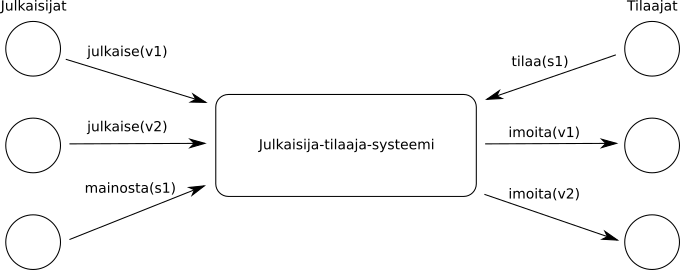
\includegraphics[width=0.9\textwidth]{pictures/publish-subscribe.png}
	\caption{Julkaisija-tilaaja-systeemi välikätenä viestien välittämisessä julkaisijoiden ja tilaajien välissä (pohjautuu kuvaan \mbox{\cite[s.~246]{distributed-systems-concepts-and-design}}).}
	\label{fig:publish-subscribe-communication}
\end{figure}

Julkaisija-tilaaja-systeemin ansiosta kommunikointi osapuolten välillä on epäsuoraa. Kommunikoinnissa osapuolten välillä on heikko tilaliitos ja vahva aikaliitos. Heikkossa tilaliitoksessa osapuolet eivät tiedä toistensa identiteettiä kuka julkaisi viestin ja kuka sen vastaanottaa. Systeemi osapuolten välissä mahdollistaa tämän. Osapuolten välillä on kuitenkin vahva aikaliitos. Jotta tilaaja saa viestin, täytyy sen olla olemassa samaan aikaan kuin julkaisijan. Yksinkertaisin julkaisija-tilaaja-systeemi on helppo implementoida yhdellä välittäjällä. Tämä voi kuitenkin tulla ongelmaksi tai pullonkaulaksi järjestelmässä, missä tiedon vaihto on nopeaa ja osapuolia on paljon tai välittäjä kaatuu kesken kaiken. Tällaisen systeemin skaalaaminen ylöspäin on vaikempaa ja vaatii hajautettua välittäjäverkkoa \cite[s.~248--249]{distributed-systems-concepts-and-design}. Lisäksi systeemin epäsuoruus tuo mukanaan kommunikointiin vaikeutta ja suoritukseen kuormaa verrattuna suoraan kommunikointiin.


\subsection{Viestijono}
Viestijono paradigmassa osapuolet kommunikoivat epäsuorasti jonon välityksellä. Joukkokommunikointi ja julkaisija-tilaaja paradigmat ovat yksi-moneen-suhde osapuolten välillä, kun taas viestijono on yksi-yhteen-suhde (engl. point-to-point). Lähettäjä lähettää viestin jonoon, josta vastaanottaja poistaa sen käsittelyyn. Viestijonon tarkoitus on puskuroida viestejä vastaanottajalle ja näin taata niiden saatavuus ja järjestys millä ajan hetkellä hyvänsä. Viestijono mahdollistaa siis osapuolten välillä heikon tila- ja aikaliitoksen. Jonon ansiosta lähettäjä ja vastaanottaja voivat olla olemassa eri aikaan \cite[s.~254]{distributed-systems-concepts-and-design}. Kuvassa \ref{fig:message-queue-communication} on esitetty viestijonosysteemin toiminta osapuolten välillä.

\begin{figure}[ht!]
	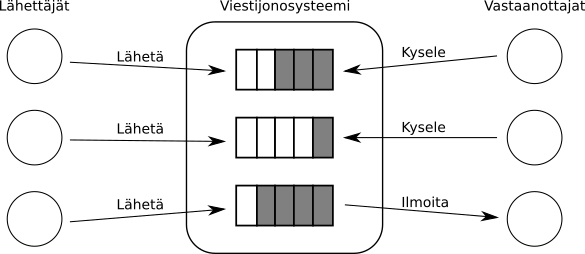
\includegraphics[width=0.9\textwidth]{pictures/message-queue.png}
	\caption{Viestijonosysteemi puskuroi viestejä lähettäjiltä vastaanottajille (pohjautuu kuvaan \mbox{\cite[s.~255]{distributed-systems-concepts-and-design}}).}
	\label{fig:message-queue-communication}
\end{figure}

Vastaanottaja voi poistaa viestejä jonosta kolmella eri periaatteella:
\begin{itemize}
	\item \emph{pysäyttävä vastaanotto} (engl. \emph{blocking receive}), joka pysäyttää kunnes viesti on saatavissa,
	\item \emph{ei pysäyttävä vastaanotto} (engl. \emph{non-blocking receive}), joka tarkistaa jonon tilan ja palauttaa viestin jos saatavilla, ja
	\item \emph{ilmoita} (engl. \emph{notify}), joka lähettää tiedon uudesta viestistä kun sellainen on saatavilla \cite[s.~254]{distributed-systems-concepts-and-design}.
\end{itemize}
Ei pysäyttävä vastaanotto on sama kuin vastaanottaja kyselisi viestejä jonosta tietyn väliajoin (engl. poll). Viestijonosysteemissä jonoa ei ole rajoitettu yhteen lähettäjään ja vastaanottajaan. Systeemissä moni lähettäjä voi lähettää viestejä samaan jonoon ja moni vastaanottaja voi vastaanottaa niitä samasta jonosta. Jonojen jonotuspolitiikka on yleensä FIFO-periaate (engl. First-In-First-Out). Moni systeemi kuitenkin tukee myös muitakin periaatteita, kuten viestien priorisointia, jossa ylemmän prioriteetin viestit käsitellään ennen alemman prioriteetin viestejä \cite[s.~120]{eugster2003many}.

Viestijonon hyvänä puolena on osapuolten heikon aikaliitoksen mahdollistaminen. Tämä mahdollistetaan sillä, että viestit jonossa ovat pysyviä (engl. persistent). Systeemi tallentaa viestit levylle, jossa ne säilyvät niin kauan kunnes vastaanottaja poistaa ne jonosta. Systeemi takaa viestien lähettämisen vastaanottajalle. Viesti tullaan lähettämään jossakin vaiheessa ja enintään kerran. Lisäksi lähetetty viesti vastaa alkuperäistä lähettäjän viestiä. \mbox{\cite[s.~255]{distributed-systems-concepts-and-design}}

Aikaisemmin käsiteltiin viestien välitystä prosessien välisessä kommunikoinnissa ja mainittiin että prosessit voivat implementoida jonon viestien vastaanottoon. Jonosysteemillä on paljon samanlaisia piirteitä tämän kanssa. Kuitenkin viestien välityksessä jonot ovat liitoksissa sen osapuoleen ja ovat implisiittisiä. Viestijonosysteemissä jonot ovat kolmannen osapuolen tarjoamia eksplisiittisiä jonoja, joka erottaa lähettäjät ja vastaanottajat toisistaan. Tämä on tärkeä ero, joka tekee viestijonosta oman epäsuoran kommunikointiparadigman. \mbox{\cite[s.~256]{distributed-systems-concepts-and-design}}

% TODO: Kirjoita tähän vielä muista jos tarpeen? (jaettu muisti, tuple space)